%Auswertung des Emissionsspektrums
\subsection{Auswertung}
Es soll das R�ntgenspektrum der Kupferanode bei drei unterschiedlichen Beschleunigungsspannungen und mit einem Ni-Filter, bei m�glichst hoher R�ntgenspannung untersucht werden.
Zum beugen der R�ntgenstrahlen wird ein Si(111)-Einkristall verwendet, der Netzebenabstand liegt bei \SI{3,1356}{\angstrom}, entnommen von \cite{si_a}.
Gescannt wird ein Winkelbereich von 15$^\circ$ bis 130$^\circ$, dabei wurden f�r die Beschleunigungsspannung Werte von
\begin{itemize}
\item U = 30kV und A = 10mA
\item U = 40kV und A = 10mA
\item U = 40kV und A = 30mA
\end{itemize}
 verwendet. Dabei ergeben sich die folgenden Plots.
 
 % Plots der Messunge f\"ur die Kupferanode mit unterschiedlichen Beschleunigungsspannungen
In Abb. \ref{fig:spektrum_1} ist das Diffraktogramm f�r U = 30kV und A = 10mA.
 
\begin{figure}[H]
	\centering
  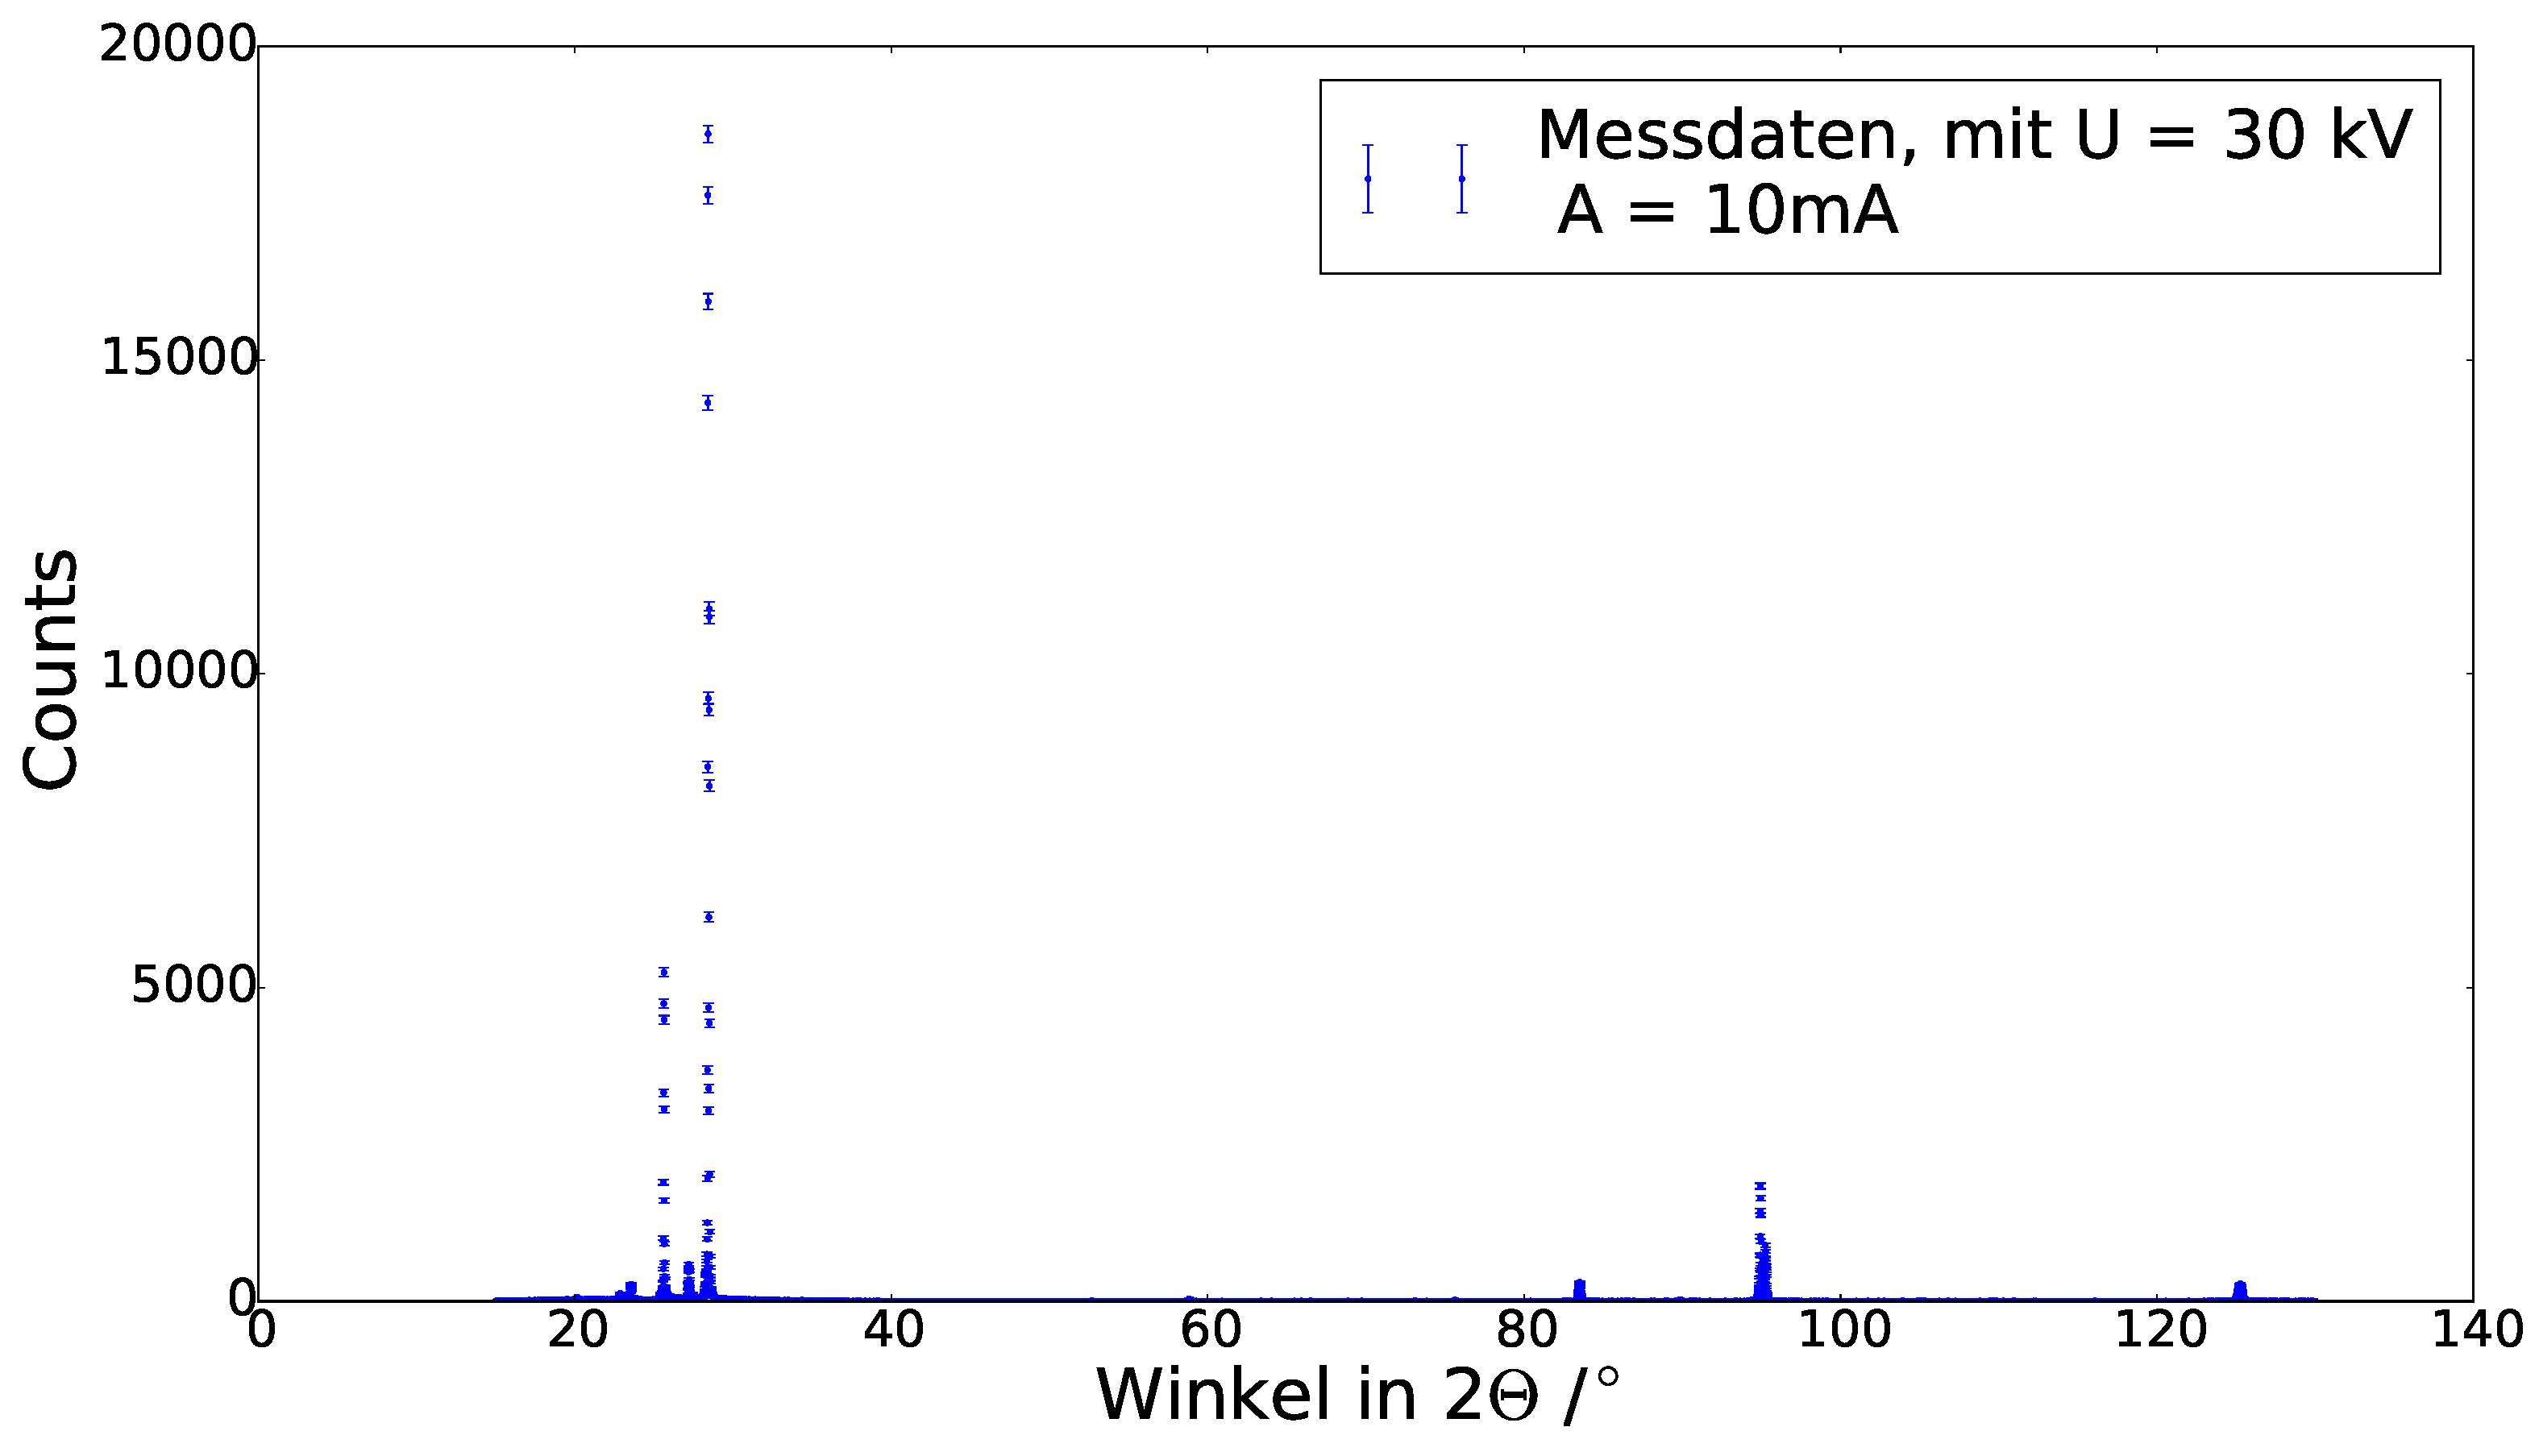
\includegraphics[scale=0.30]{spektrum_1.pdf}
	\caption{Diffraktogramm bei 30kV Beschleunigungsspannung und einem Anodenstrom von 10mA}
	\label{fig:spektrum_1}
\end{figure}

In Abb. \ref{fig:spektrum_2} ist das Diffraktogramm f�r U = 40kV und A = 10mA.
 
\begin{figure}[H]
	\centering
  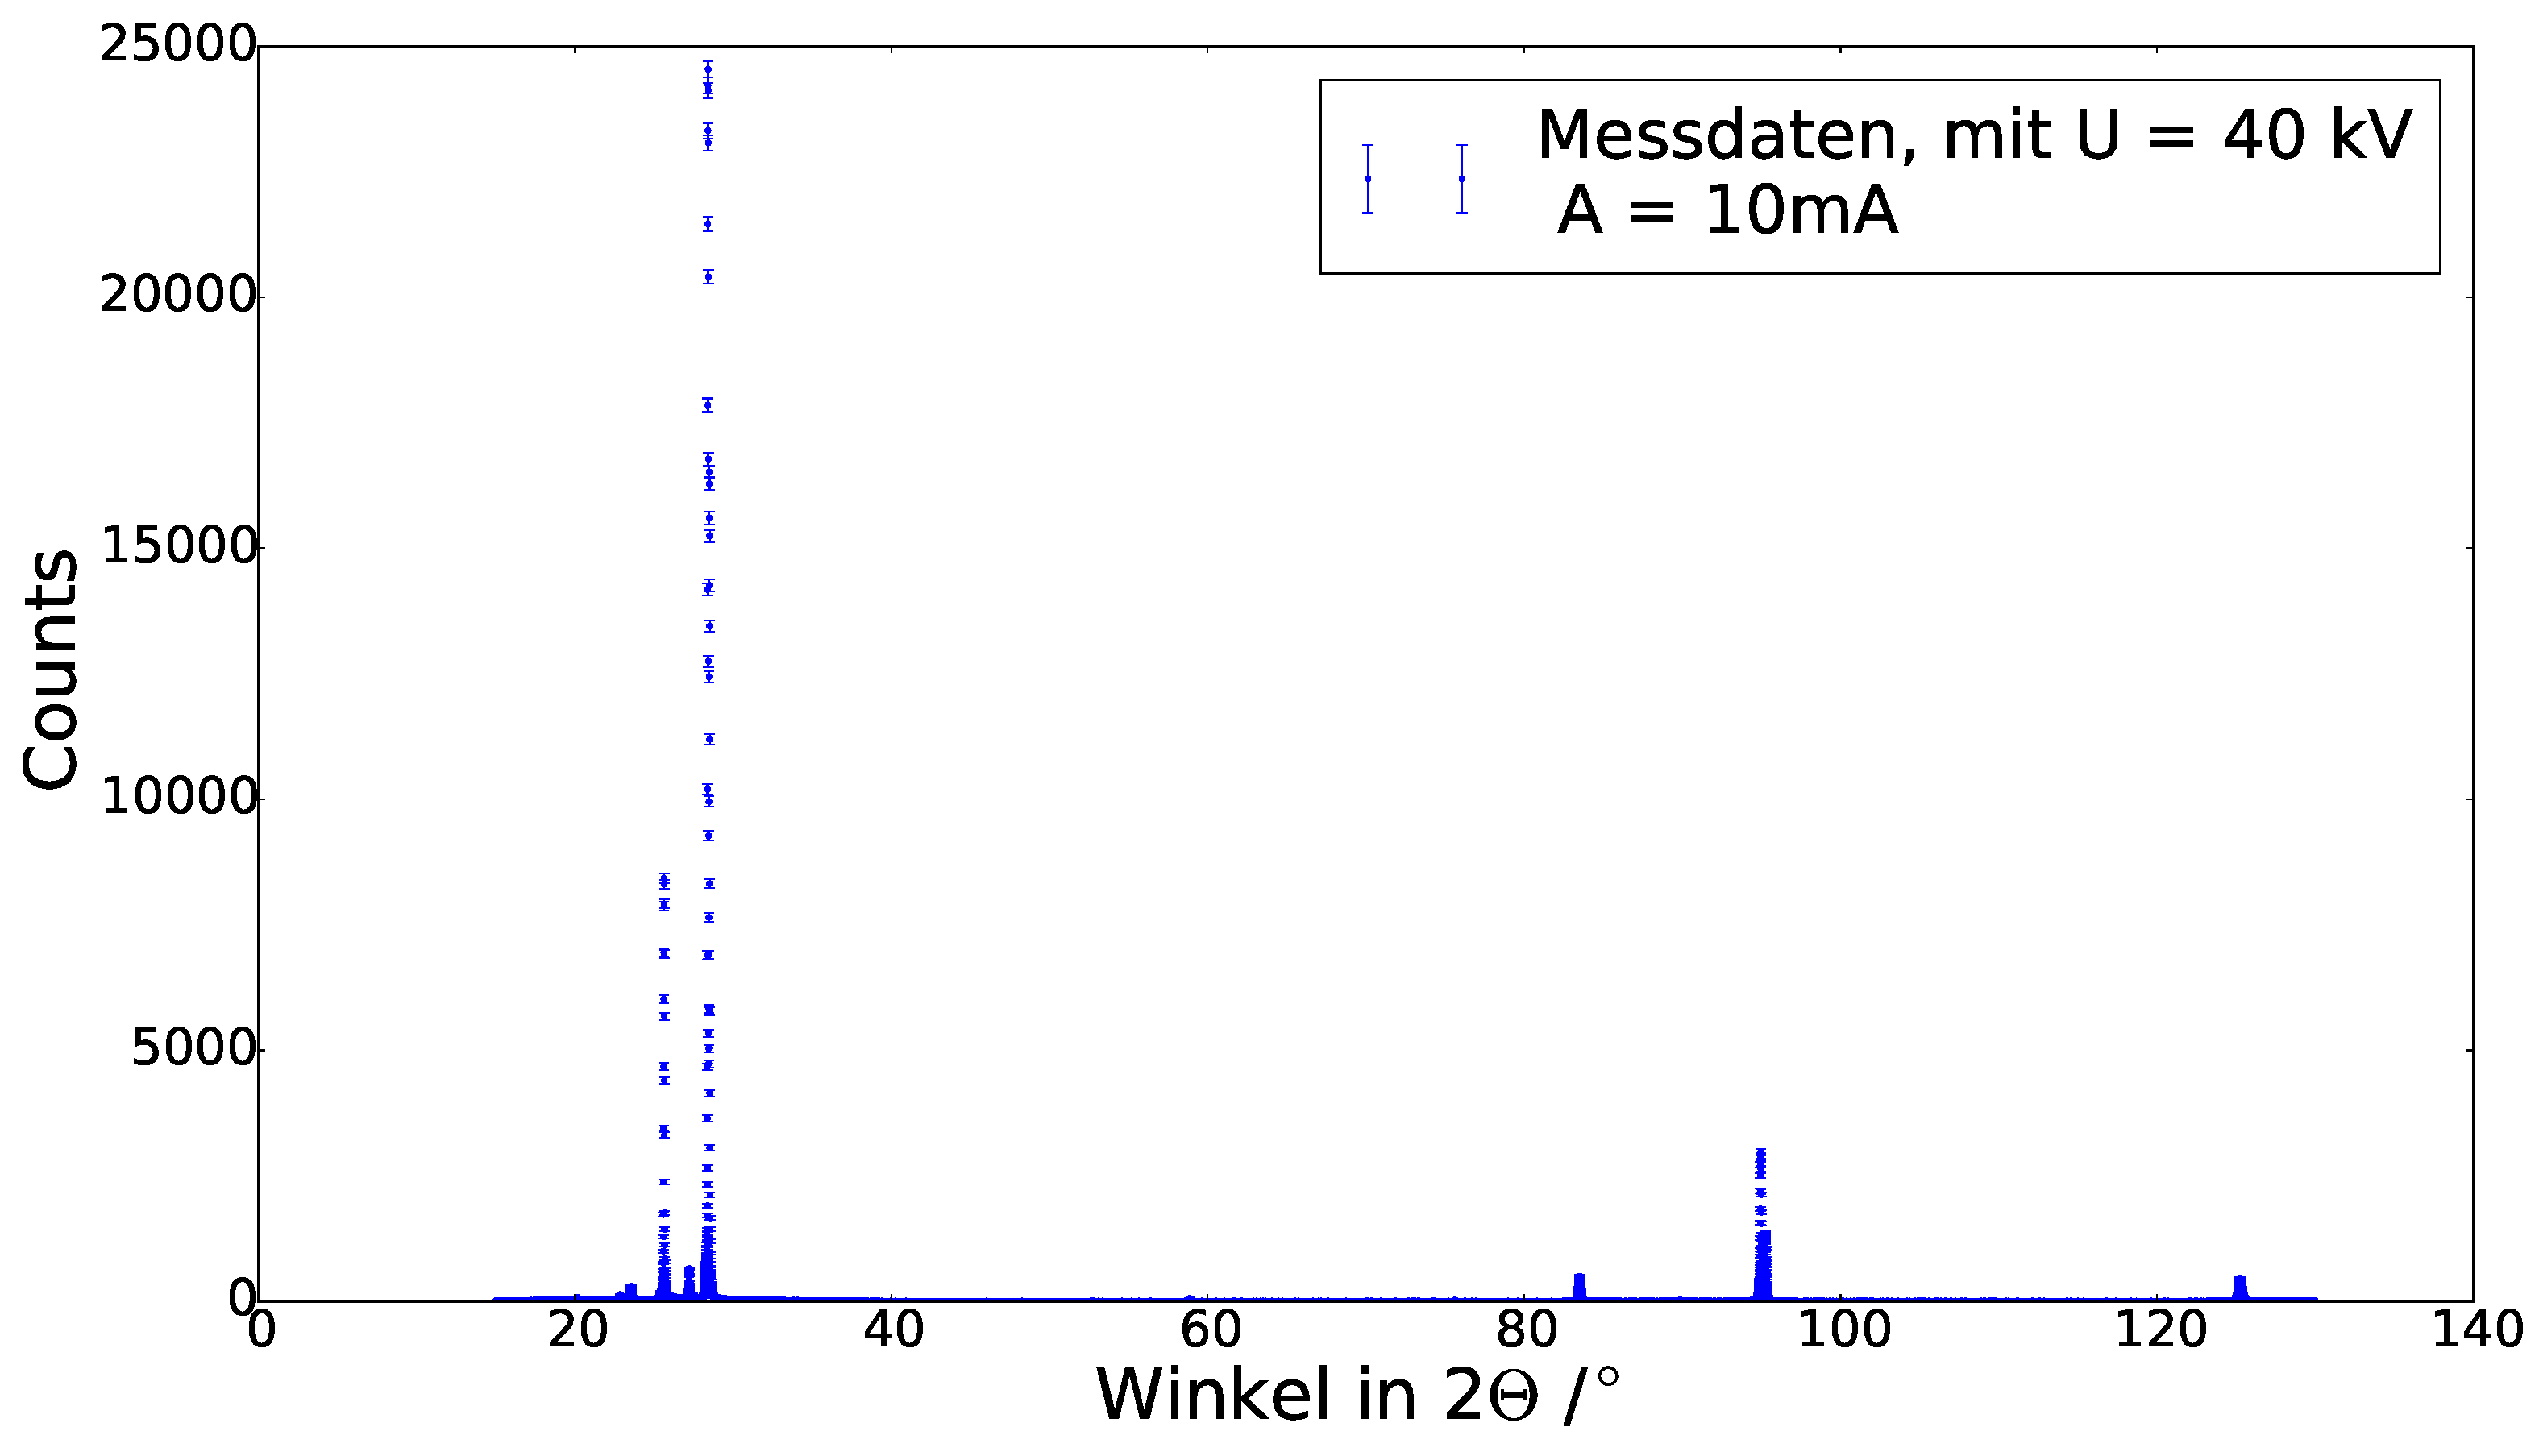
\includegraphics[scale=0.30]{spektrum_2.pdf}
	\caption{Diffraktogramm bei 40kV Beschleunigungsspannung und einem Anodenstrom von 10mA}
	\label{fig:spektrum_2}
\end{figure}

In Abb. \ref{fig:spektrum_3} ist das Diffraktogramm f�r U = 40kV und A = 30mA.

\begin{figure}[H]
	\centering
  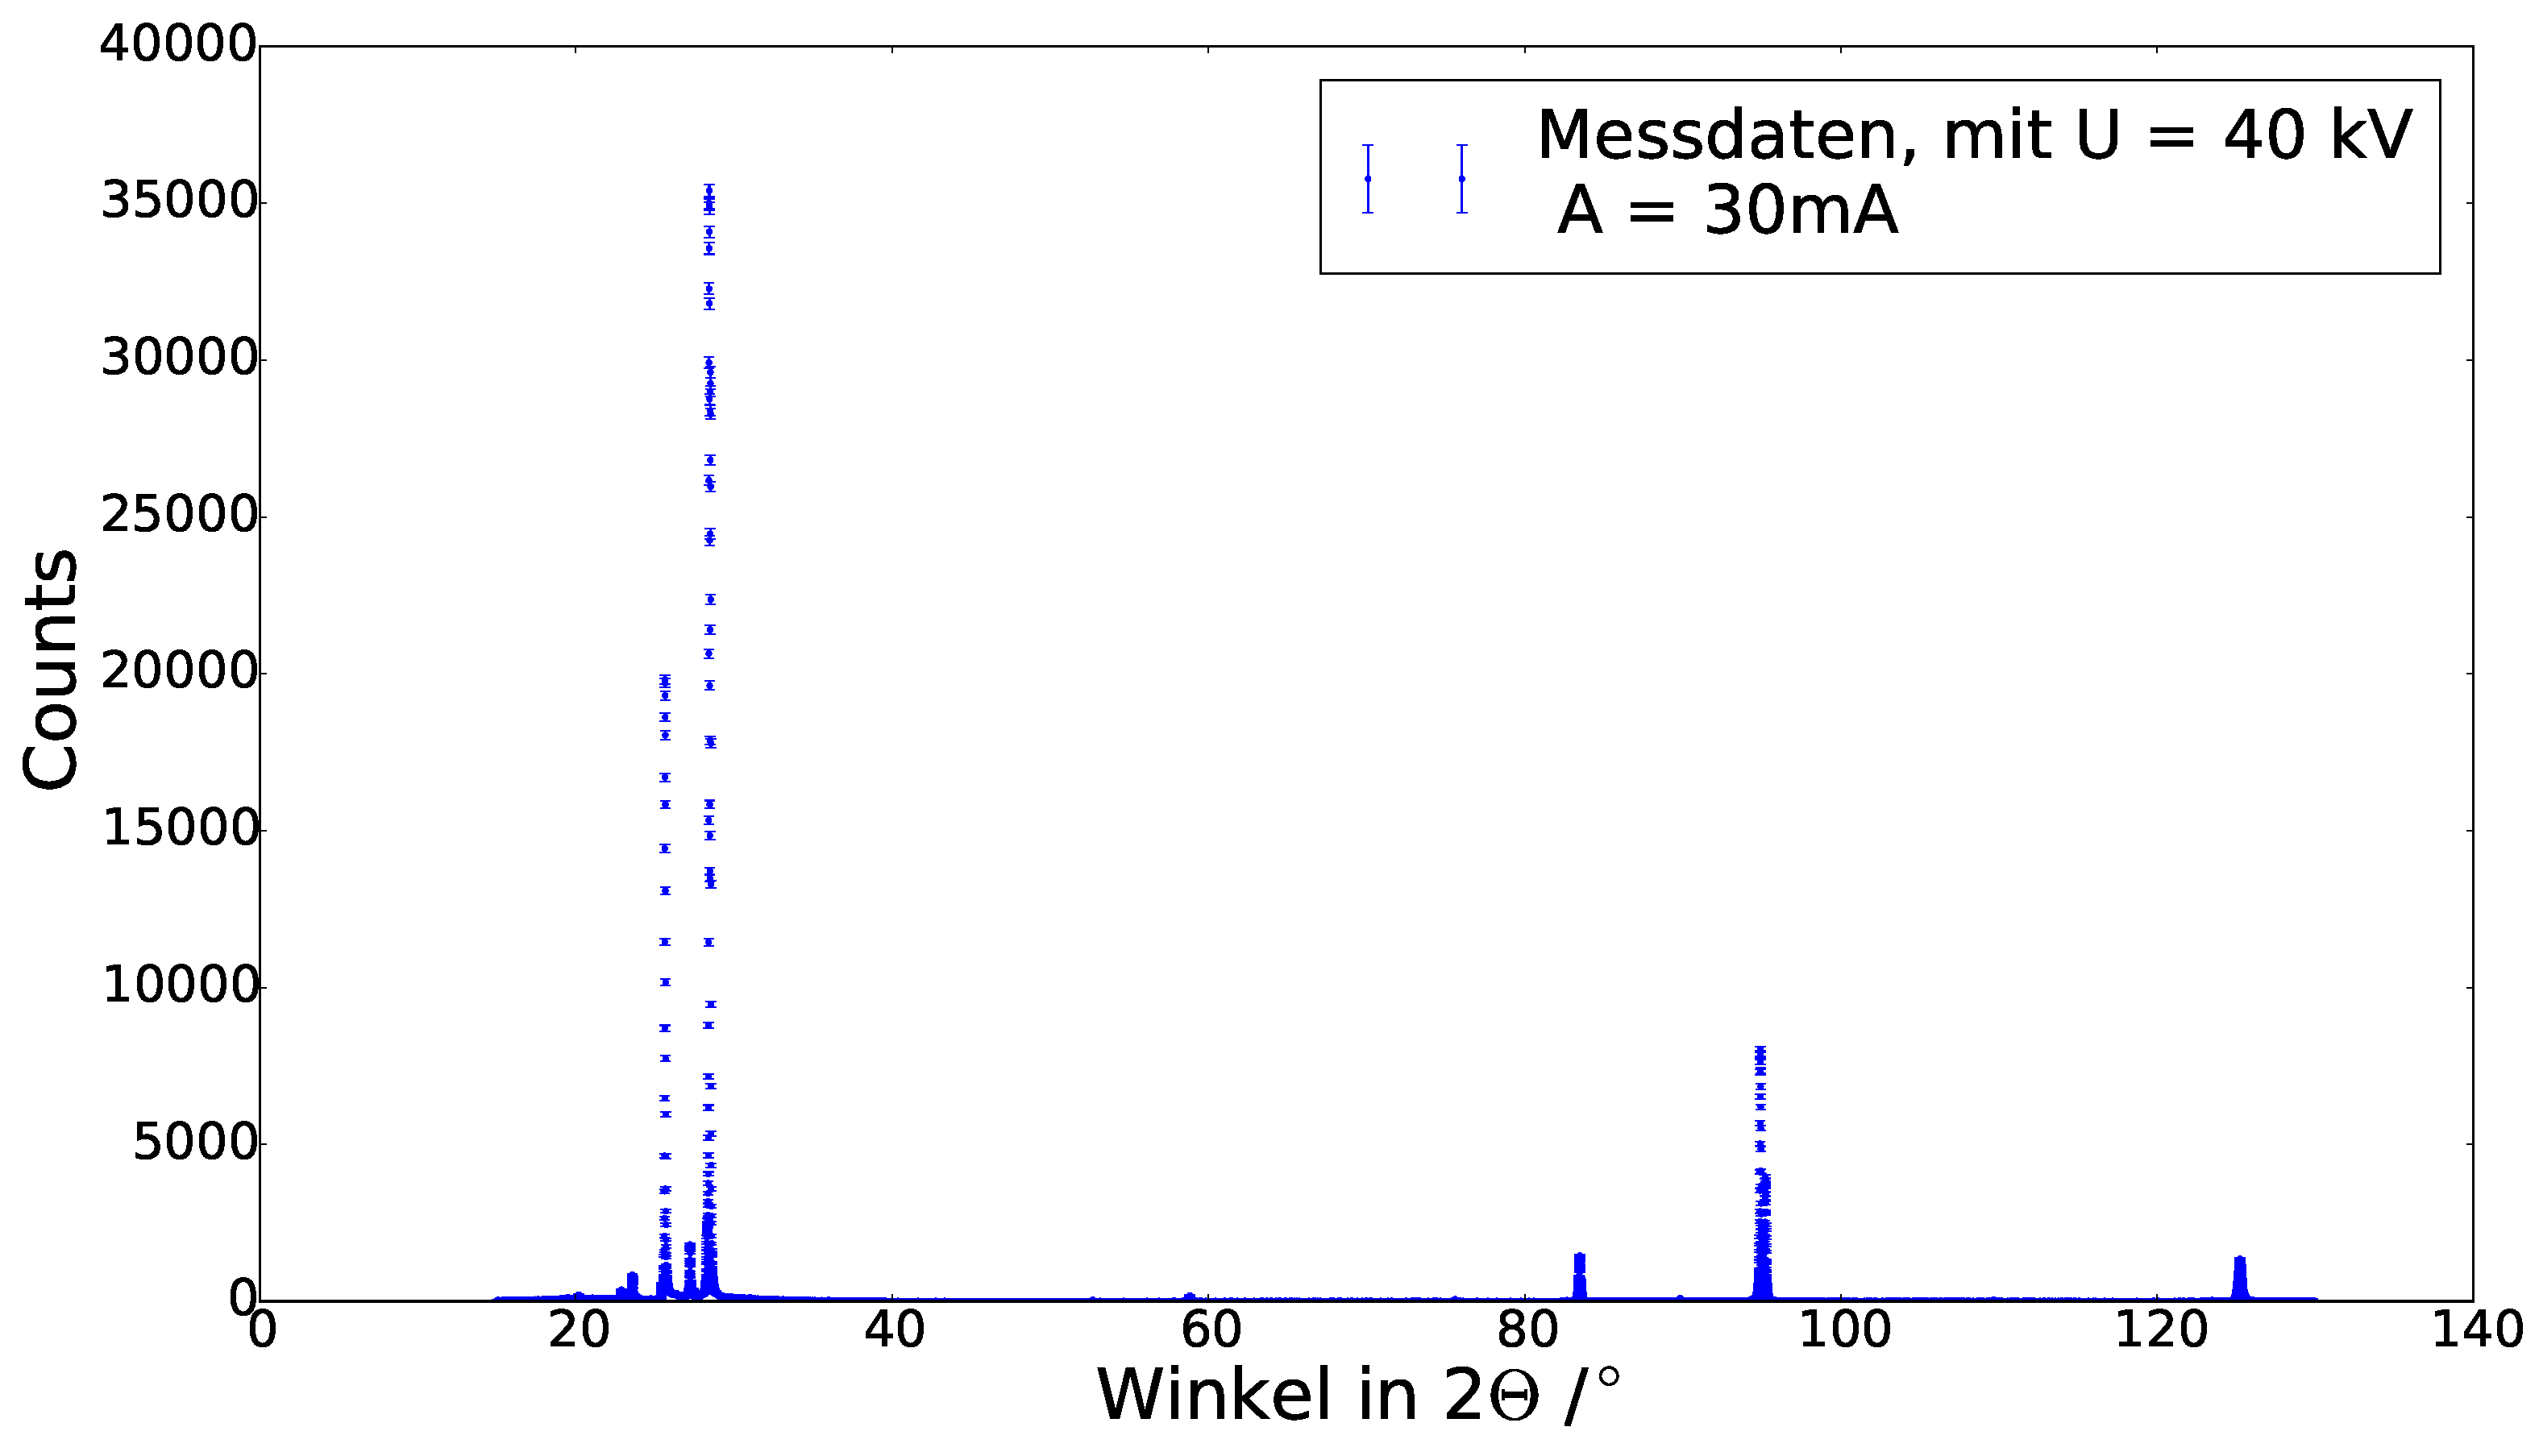
\includegraphics[scale=0.30]{spektrum_3.pdf}
	\caption{Diffraktogramm bei 40kV Beschleunigungsspannung und einem Anodenstrom von 30mA}
	\label{fig:spektrum_3}
\end{figure}
 

Es ist deutlich zu erkennen, das bei steigender Beschleunigungsspannung und Strom die Anzahl der Counts gr��er werden und so die Peaks deutlich von dem Untergrund zu unterscheiden sind. Um Informationen �ber den Winkel und die Intensit�t zu erhalten, werden die Peaks mit der Voigtverteilung gefittet. Aus den Fitparametern kann die Intensit�t der einzelnen Peaks bestimmt und verglichen werden. Der Fit f�r U=30kV und A=10mA ist in Abb. \ref{fig:30_10_fit} zu sehen, die Fitparameter ergaben sich die Werte in Tabelle \ref{tab:30_10_fit}. Alle weiteren Peaks wurde nach dem selben verfahren bestimmt.

\begin{figure}[H]
	\centering
  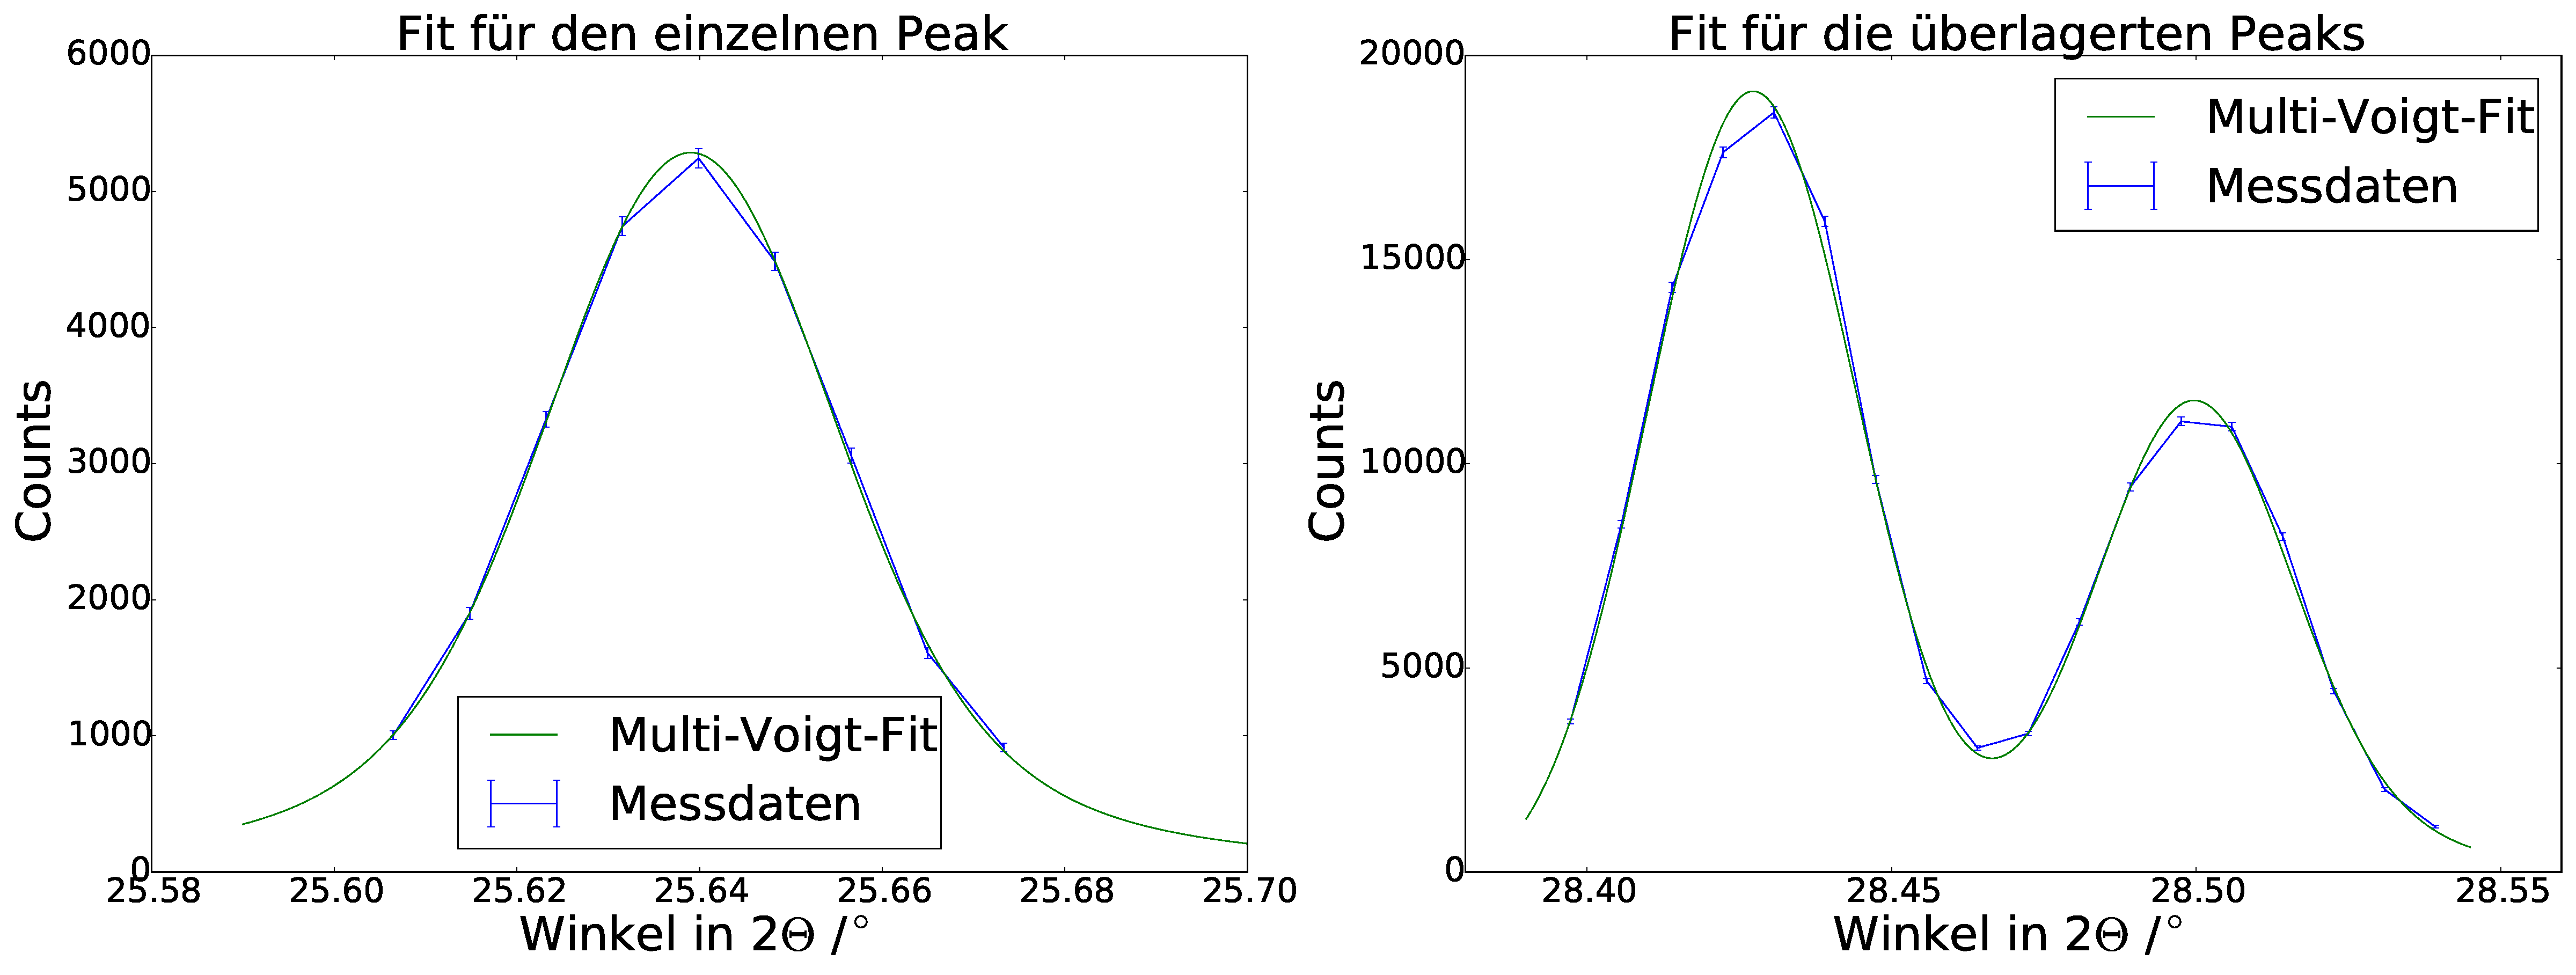
\includegraphics[scale=0.2]{30_10_voigt.pdf}
	\caption{Diffraktogramm bei 40kV Beschleunigungsspannung und einem Anodenstrom von 30mA}
	\label{fig:30_10_fit}
\end{figure}


\begin{table}[H]
\centering
\caption{Fitparameter f�r eine Beschleunigungsspannung von 30kV und einem Anodenstrom von 10mV}
\label{tab:30_10_fit}
\begin{tabular}{|c|c|c|c|c|c|c|}
\hline Peak & Paramter & Center & Amplitude & Sigma & Gamma & $\chi_{red}^2$ \\ 
\hline 1 & Wert & 25,6390 $\pm$ 0,0001 & 260 $\pm$ 5 & 0,0124 $\pm$ 0,0007 & 0,008 $\pm$ 0,001 & 1,08 \\ 
\hline 2 & Wert & 28,4278 $\pm$ 0,0007  & 790 $\pm$ 96 & 0,0187 $\pm$ 0,003 & -0,003 $\pm$ 0,006 & 16,11 \\ 
\hline 3 & Wert & 28,4996 $\pm$ 0,0007 & 425 $\pm$ 128 & 0,021 $\pm$ 0,006 & -0,01 $\pm$ 0,01 & 16,11 \\ 
\hline 
\end{tabular} 
\end{table}

\subsubsection{Verh�ltnisse}
Aus den bestimmten Peaks sollen die Verh�ltnisse der Cu-Linien und der Ordnungen unter einander. F�r den Voigt-Fit die eingebaute Funktion des Pythonpackages lmfit (cite) verwendet. Die Voigtverteilung wird �ber ein normiertes Intergral bestimmt, worduch der Fit Parameter f�r die Amplitude f�r die Verh�ltnisbestimmung verwendet werden. Die mit den Fits bestimmten Amplituden sind in Tabelle \ref{tab:wichtige_parameter} zu sehen.

\begin{table}[H]
\centering
\caption{Bestimmte Winkel und Amplituden f�r die verschiedenen Beschleunigungsspannungen und Anodenstr�me}
\label{tab:wichtige_parameter}
\begin{tabular}{|c|c|c|c|c|}
\hline Beschleunigunsspannung und Anodenstrom & Ordnung & Linie & Winkel & Amplitude \\ 
\hline U = 30 kV, A = 10mA & 1 & $K_{\alpha_1}$ & 28,4278 $\pm$ 0,0007 & 790 $\pm$ 96 \\ 
\hline  &  & $K_{\alpha_2}$ & 28,4996 $\pm$ 0,0007 & 425 $\pm$ 128 \\ 
\hline  &  & $K_\beta$ & 25,639 $\pm$ 0,001 & 260 $\pm$ 5 \\ 
\hline  & 3 & $K_{\alpha_1}$ & 94,933 $\pm$ 0,004 & 155 $\pm$ 2 \\ 
\hline  &  & $K_{\alpha_2}$ & 94,2453 $\pm$ 0,0006 & 76 $\pm$ 2 \\ 
\hline  &  & $K_\beta$ & 83,5022 $\pm$ 0,0008 & 37 $\pm$ 1 \\ 
\hline U = 40 kV, A = 10 mA & 1 & $K_{\alpha_1}$ & 28,4282 $\pm$ 0,0003 & 1149 $\pm$ 52 \\ 
\hline  &  & $K_{\alpha_2}$ & 28,5008 $\pm$ 0,0003 & 654 $\pm$ 75 \\ 
\hline  &  & $K_\beta$ & 25,5400 $\pm$ 0.0001 & 425 $\pm$ 6 \\ 
\hline  & 3 & $K_{\alpha_1}$ & 94,9336 $\pm$ 0,0003 & 245 $\pm$ 2 \\ 
\hline  &  & $K_{\alpha_2}$ & 95,2448 $\pm$ 0,0004 & 122 $\pm$ 2 \\ 
\hline  &  & $K_\beta$ & 83,5043 $\pm$ 0,0006 & 57 $\pm$ 2 \\ 
\hline U = 40 kV, a = 30 mA & 1 & $K_{\alpha_1}$ & 28,433 $\pm$ 0,001 & 1046 $\pm$ 873 \\ 
\hline  &  & $K_{\alpha_2}$ & 28,507 $\pm$ 0,001 & 1814 $\pm$ 613 \\ 
\hline  &  & $K_\beta$ & 25,6452 $\pm$ 0,0001 & 498 $\pm$ 158 \\ 
\hline  & 3 & $K_{\alpha_1}$ & 94,9398 $\pm$ 0,0002 & 771 $\pm$ 6 \\ 
\hline  &  & $K_{\alpha_2}$ & 95,2518 $\pm$ 0,0003 & 362 $\pm$ 4 \\ 
\hline  &  & $K_\beta$ & 83,5110 $\pm$ 0,0004 & 184 $\pm$ 4 \\ 
\hline 
\end{tabular} 
\end{table}

Das Verh�ltnis wir nach Gl. \ref{eqn:verh�ltniss} bestimmt, der Fehler ergibt sich dabei nach Gl. \ref{eqn:delta_verh�ltniss}.

\begin{align}
\label{eqn:verh�ltniss}
V = \frac{A_1}{A_2}
\end{align}

\begin{align}
\label{eqn:delta_verh�ltniss}
\Delta V = \sqrt{\left( \frac{\Delta A_1}{A_2} \right)^2 + \left( \frac{\Delta A_2 A_1}{A_2^2} \right)^2}
\end{align}

 Aus den Amplituden in Tabelle \ref{tab:wichtige_parameter} ergeben sich die Verh�ltnisse unter den Ordnungen in Tabelle \ref{tab:verh�ltniss_ordnung}. Die Verh�ltnisse bei unterschiedlichen Beschleunigungsspannungen und Anodenstr�men sind in Tabelle \ref{tab:verh�ltniss_messung} aufgetragen.

\begin{table}[H]
\centering
\caption{Verh�ltniss der Peaks bei unterschiedlicher Ordnung, dabei wird die Amplitude des Peaks erster Ordnung durch den der dritten geteilt}
\label{tab:verh�ltniss_ordnung}
\begin{tabular}{|c|c|c|}
\hline Anodenspannung und Anodenstrom & Linie  & Verh�ltniss \\ 
\hline U = 30 kV, A = 10 mA & $K_\beta$ & 7,027 $\pm$ 0,2 \\ 
\hline  & $K_{\alpha_1}$ &  5,1 $\pm$ 0,6 \\ 
\hline  & $K_{\alpha_2}$ & 6 $\pm$ 2 \\ 
\hline U = 40 kV, A = 10 mA & $K_\beta$ & 7,4 $\pm$ 0,3 \\ 
\hline  & $K_{\alpha_2}$ & 4,7 $\pm$ 0,2 \\ 
\hline  & $K_{\alpha_2}$ & 5,4 $\pm$ 0,6 \\ 
\hline U = 40 kV, A = 30 mA & $K_\beta$ & 2,7 $\pm$ 0,8 \\ 
\hline  & $K_{\alpha_2}$ & 1 $\pm$ 1 \\ 
\hline  & $K_{\alpha_2}$ & 5 $\pm$ 2 \\ 
\hline 
\end{tabular} 
\end{table}


\begin{table}[H]
\centering
\caption{Verh�ltniss der Peaks bei unterschiedlichen Beschleunigungsspannungen und Anodenstr�men, dabei wird die Amplitude des Peaks erster Ordnung durch den der dritten geteilt}
\label{tab:verh�ltniss_messung}
\begin{tabular}{|p{3,5cm}|c|c|c|c|}
\hline Beschleunigungs- spannung  und Anodenstrom &  Ordnung & $K_\beta$ & $K_{\alpha_2}$ & $K_{\alpha_2}$ \\ 
\hline 30 10 / 40 10 & 1 & 0,61 $\pm$ 0,01 & 0,69 $\pm$ 0,09 & 0,6 $\pm$ 0,2 \\ 
\hline  & 3 & 0,650 $\pm$ 0,003 & 0,63 $\pm$ 0,01 & 0,62 $\pm$ 0,02 \\ 
\hline 30 10 / 40 30 & 1 & 0,5 $\pm$ 0,2 & 0,8 $\pm$ 0,6 & 0,2 $\pm$ 0,1 \\ 
\hline  & 3 & 0,201 $\pm$ 0,007 & 0,218 $\pm$ 0,003 & 0,210 $\pm$ 0,006 \\ 
\hline 40 10 / 40 30 & 1 & 0,9 $\pm$ 0,3 & 1,1 $\pm$ 0,9 & 0,36 $\pm$ 0,01 \\ 
\hline  & 3 & 0,31 $\pm$ 0,01 & 0,3446 $\pm$ 0,0004 & 0,337 $\pm$ 0,007 \\ 
\hline 
\end{tabular} 
\end{table}

\subsubsection{Abschw�chung durch den Ni-Filter}
Es soll die Abschw�chung der K$_\beta$-Linie und das Signal-zu-Rausch Verh�ltniss der K$_{\alpha_{1,2}}$-Linie und deren Energie und Energiebreite bestimmt werden.
Mit Verwendung des Filters ergibt sich das Diffrakogramm in Abbildung ??.

%Diffraktogramme mit Fits einf�gen

Es ergibt sich eine Countrate von ?? mit Ni-Filter und ein Count von ?? ohne Ni-Filter. Daraus ergibt sich ein Verh�ltnis von ??.
Das Signal-zu-Rauschverh�ltnis (SNR) wir in [dB] berechnet:

\begin{align}
SNR = 10 \cdot lg \left( \frac{I_{max}}{I_{rausch}} \right)
\end{align}

\subsubsection{Netzebenabstand Si(331)}
Der Si(111)-Einkristall wird nun gegen einen Si(331)-Einkristall ausgetauscht.
Mit den zuvor bestimmten Energien der Cu-Linien soll nach Gleichung ?? der Netzebenabstand bestimmt werden, der Fehler wird mit Gleichung ?? berechnet.
Die Peaks wurden wie zuvor mit der Gau�verteilung gefittet.

%Plot der Peaks mit Fit 

Aus den Messdaten ergeben sich die Werte in Tabelle ??

\begin{table}[H]
\label{tab:si(331)}
\caption{In der Tabelle sind die Ergebnisse zur Bestimmung des Netzebenabstandes von Si(331)}
\centering
\begin{tabular}{|c|c|c|}
\hline Werte & K$_{\alpha_1}$ & K$_{\alpha_2}$ \\ 
\hline 2$\theta [^\circ]$ &  &  \\ 
\hline $\Delta 2\theta [^\circ]$ &  &  \\ 
\hline E[eV] &  &  \\ 
\hline $\Delta$E[eV] &  &  \\ 
\hline d$[\SI{}{\angstrom}]$ &  &  \\ 
\hline $\Delta$d$[\SI{}{\angstrom}]$ &  &  \\ 
\hline 
\end{tabular} 
\end{table}

%Vergleich mit den Literaturwerten


\subsubsection{Netzebenabstand Ge(111)}
Es soll ein Ge(111)-Einkristall untersucht werden, dabei wird wie zuvor vorgegangen.

Aus den Messdaten ergeben sich die Werte in Tabelle ??

\begin{table}[H]
\label{tab:ge(111)}
\caption{In der Tabelle sind die Ergebnisse zur Bestimmung des Netzebenabstandes von Ge(111)}
\centering
\begin{tabular}{|c|c|c|}
\hline Werte & K$_{\alpha_1}$ & K$_{\alpha_2}$ \\ 
\hline 2$\theta [^\circ]$ &  &  \\ 
\hline $\Delta 2\theta [^\circ]$ &  &  \\ 
\hline E[eV] &  &  \\ 
\hline $\Delta$E[eV] &  &  \\ 
\hline d$[\SI{}{\angstrom}]$ &  &  \\ 
\hline $\Delta$d$[\SI{}{\angstrom}]$ &  &  \\ 
\hline 
\end{tabular} 
\end{table}


%Vergleich mit den Literaturwerten



